\documentclass[12pt]{article}
%\documentclass[12pt,legalpaper]{article}
%\documentclass[14pt,legalpaper]{extarticle}
\usepackage{fullpage}
\usepackage{amsmath,amssymb}
\usepackage{mathptmx}
\usepackage{fancyhdr}
\usepackage{lastpage}
\usepackage{multicol}
\usepackage{graphicx}
\usepackage[aux]{rerunfilecheck}
\usepackage[rflt]{floatflt}

%\setlength{\textheight}{11.5in}

\reversemarginpar

\newcommand{\myimp}{\Rightarrow}
\newcommand{\myiff}{\Leftrightarrow}
\newcommand{\mynot}{\neg}
\newcommand{\myor}{\vee}
\newcommand{\myand}{\wedge}
\newcommand{\ds}{\displaystyle}

\DeclareSymbolFont{AMSb}{U}{msb}{m}{n}
\DeclareMathSymbol{\N}{\mathbin}{AMSb}{"4E}
\DeclareMathSymbol{\Z}{\mathbin}{AMSb}{"5A}
\DeclareMathSymbol{\R}{\mathbin}{AMSb}{"52}
\DeclareMathSymbol{\Q}{\mathbin}{AMSb}{"51}
\DeclareMathSymbol{\I}{\mathbin}{AMSb}{"49}
\DeclareMathSymbol{\C}{\mathbin}{AMSb}{"43}

\pagestyle{fancy}
\lhead{MATH 110 200930                                                     \\ 
  Sample Final Examination 3 \hspace{0.75in} Page\ \thepage\ of \pageref{LastPage}  \\ 
  Time: 3 hours                                                            \\
  \quad                                                                      }
%\chead{\quad                                                              \\ 
%       Page\ \thepage\ of \pageref{LastPage}                              \\ 
%	\quad                                                                }
\chead{}
\rhead{Name: \underline{\hspace{2in}}        \\ 
       Student \#: \underline{\hspace{2in}}  \\ 
       Section: \underline{\hspace{2in}}     \\
       \quad                                   }
\cfoot{}
\addtolength{\headheight}{\baselineskip}
\addtolength{\headheight}{\baselineskip}
\addtolength{\headheight}{\baselineskip}
\addtolength{\headheight}{\baselineskip}
\renewcommand{\headrulewidth}{0pt}
\fancypagestyle{plain}{%
  \lhead{}
  \chead{FIRST NATIONS UNIVERSITY OF CANADA                \\
    DEPARTMENT OF SCIENCE \\
    MATH 110 200930 \\
  }
  \rhead{}
  \cfoot{Page\ \thepage\ of \pageref{LastPage}}
}

\title{Sample Final Examination 3}
\author{Dr.\ D.\ Stanley, Dr.\ R.\ McIntosh, Dr.\ S.\ Panafidin, 
  Dr.\ R.\ Floricel, Dr.\ F.\ Labropulu, Ms.\ S.\ Lisawadi}

\begin{document}
\thispagestyle{plain}
%\maketitle

\begin{center}
  \LARGE{MATH 110 200930 Sample Final Examination 3}
\end{center}

\begin{flushleft}
\quad\\
Time:  3 hours                  \hfill       Name: \underline{\hspace{2in}}  \\
Instructors:                    \hfill Student \#: \underline{\hspace{2in}}  \\
\quad Dr. Edward Doolittle      \hfill    Section: \underline{\hspace{2in}}  \\
\end{flushleft}


\noindent
You have 3 hours to do each of the following questions.
The test is worth a total of 100 marks.
Please\marginpar{\footnotesize{(marks)}} justify your conclusions and
show all your work.
A non-programmable calculator of the type mentioned in the course outline
is permitted; no other aids are permitted.
%Use the backs of the pages for rough work.

\begin{enumerate}
\item Find\marginpar{\footnotesize{(12)}}
  $\ds\frac{dy}{dx}$ in each of the following cases.  (You do not have to
  simplify your answers.)
  \begin{enumerate}
  \item $\ds y=\frac{1}{x^{1/3}} - x^7 + \cos x$
\vfill
  \item $\ds y=\frac{\sin^2(3x)}{x^3-3}$
\vfill
  \item $\ds 2y^4 + x^2 + xy^2 = 4$
\vfill
  \item $\ds y=\int_1^x \frac{\cos t}{t} \; dt$
\vfill
  \end{enumerate}
\newpage
\item Evaluate\marginpar{\footnotesize{(12)}}
  the following limits if they exist.
  \begin{enumerate}
  \item $\ds \lim_{x\to 0} 
    \frac{\sin 3x}{2x}$
\vfill
  \item $\ds \lim_{x\to\infty} \frac{4x^4+5}{(2-x^2)(2x^2+1)}$
\vfill
  \item $\ds \lim_{x\to 4} \frac{x^2-4x}{x^2-3x-4}$
\vfill
  \item $\ds \lim_{h\to 0} \frac{\sqrt{9+h}-3}{h}$
\vfill
  \end{enumerate}
\newpage
  \begin{center}
    \includegraphics[width=6in]{grph.eps}%
  \end{center}
\item Consider\marginpar{\footnotesize{(6)}} 
  the above graph of the function $f$.
  \begin{enumerate}
  \item List all $x$ for which $f$ fails to be continuous.
\vfill
  \item List all $x$ for which $f$ fails to be differentiable.
\vfill
  \end{enumerate}
\newpage
\item Use\marginpar{\footnotesize{(6)}} 
  the Intermediate Value Theorem to show that $\ds f(x)=x^3-2x-1$ must have
  at least one root in the interval $[1,2]$.
\vfill
\item Find\marginpar{\footnotesize{(10)}}
  the equation of the tangent line to the curve $\ds (x-y)^2+\frac{1}{xy}=1$
  at the point $(1,1)$.
\vfill
\vfill
\vfill
\newpage
\item Bus\marginpar{\footnotesize{(10)}} 
  station A is located 100 km west of bus station B.  At noon, a bus leaves
  bus station A driving south at 70 km/h and a second bus leaves bus station
  B driving north at 50 km/h.  How fast is the distance between buses changing
  at 2:00 pm?
\newpage
\item Let\marginpar{\footnotesize{(12)}}
  $\ds f(x)=\frac{2-x}{\sqrt{x^2+2}}$.  Then
  $\ds f'(x) = \frac{-2x-2}{(x^2+2)^{3/2}}$ and
  $\ds f''(x) = \frac{2(x+2)(2x-1)}{(x^2+2)^{5/2}}$.
  \begin{enumerate}
  \item Identify all (if any) \\
    intercepts \hrulefill \\
    local maxima \hrulefill \\
    local minima \hrulefill \\
    points of inflection \hrulefill \\
    asymptotes \hrulefill 
  \item Determine the intervals on which $f$ is \\
    increasing \hrulefill \\
    decreasing \hrulefill \\
    concave up \hrulefill \\
    concave down \hrulefill \\
    Use the space below to show your work for parts (a) and (b).  If more space
    is required use the back of the facing page and indicate that you have
    done so.
\vfill
  \end{enumerate}
\newpage
\addtocounter{enumi}{-1}
\item (continued)
  \begin{enumerate}
  \setcounter{enumii}{2}
  \item Use the information in parts (a) and (b) to sketch a graph of $f$.
  \end{enumerate}
\vfill
\newpage
\item A\marginpar{\footnotesize{(10)}} 
  veterinarian has 100 feet of fencing and wishes to construct six identical
  dog kennels by first building a fence around a rectangular region, and
  then subdividing that region into six smaller rectangles by placing five
  fences parallel to one of the sides.  What are the dimensions of the
  region that maximize the total area? 
\vfill
\newpage
\item Find\marginpar{\footnotesize{(10)}}
  the area of the region bounded by the curves
  $y=1-x^2$ and $y=x^2-3$.
\vfill
\newpage
\item Evaluate\marginpar{\footnotesize{(12)}} 
  the following integrals.
  \begin{enumerate}
  \item $\ds \int \frac{x+2\sqrt{x}+1}{\sqrt{x}} \; dx$
\vfill
  \item $\ds \int_0^{1/2} t \sin(2\pi t^2) \; dt$
\vfill
  \item $\ds \int \frac{\cos(\sqrt{\theta})}{\sqrt{\theta}} \; d\theta$
\vfill
  \item $\ds \int_0^1 x \sqrt{1-x^2} \; dx$
\vfill
  \end{enumerate}
\end{enumerate}
\end{document}

